\documentclass{article}

\usepackage{graphicx}
\usepackage{tikz}
\usepackage{tikzsymbols}
\usetikzlibrary{calc,patterns,shapes.geometric}
\pagestyle{empty}
\usepackage[margin=0pt]{geometry}
\geometry{papersize={14in,12in}}

\def\centerarc[#1](#2)(#3:#4:#5){\draw[#1] ($(#2)+({#5*cos(#3)},{#5*sin(#3)})$) arc (#3:#4:#5);}

\begin{document}
	\begin{figure}
		\centering
		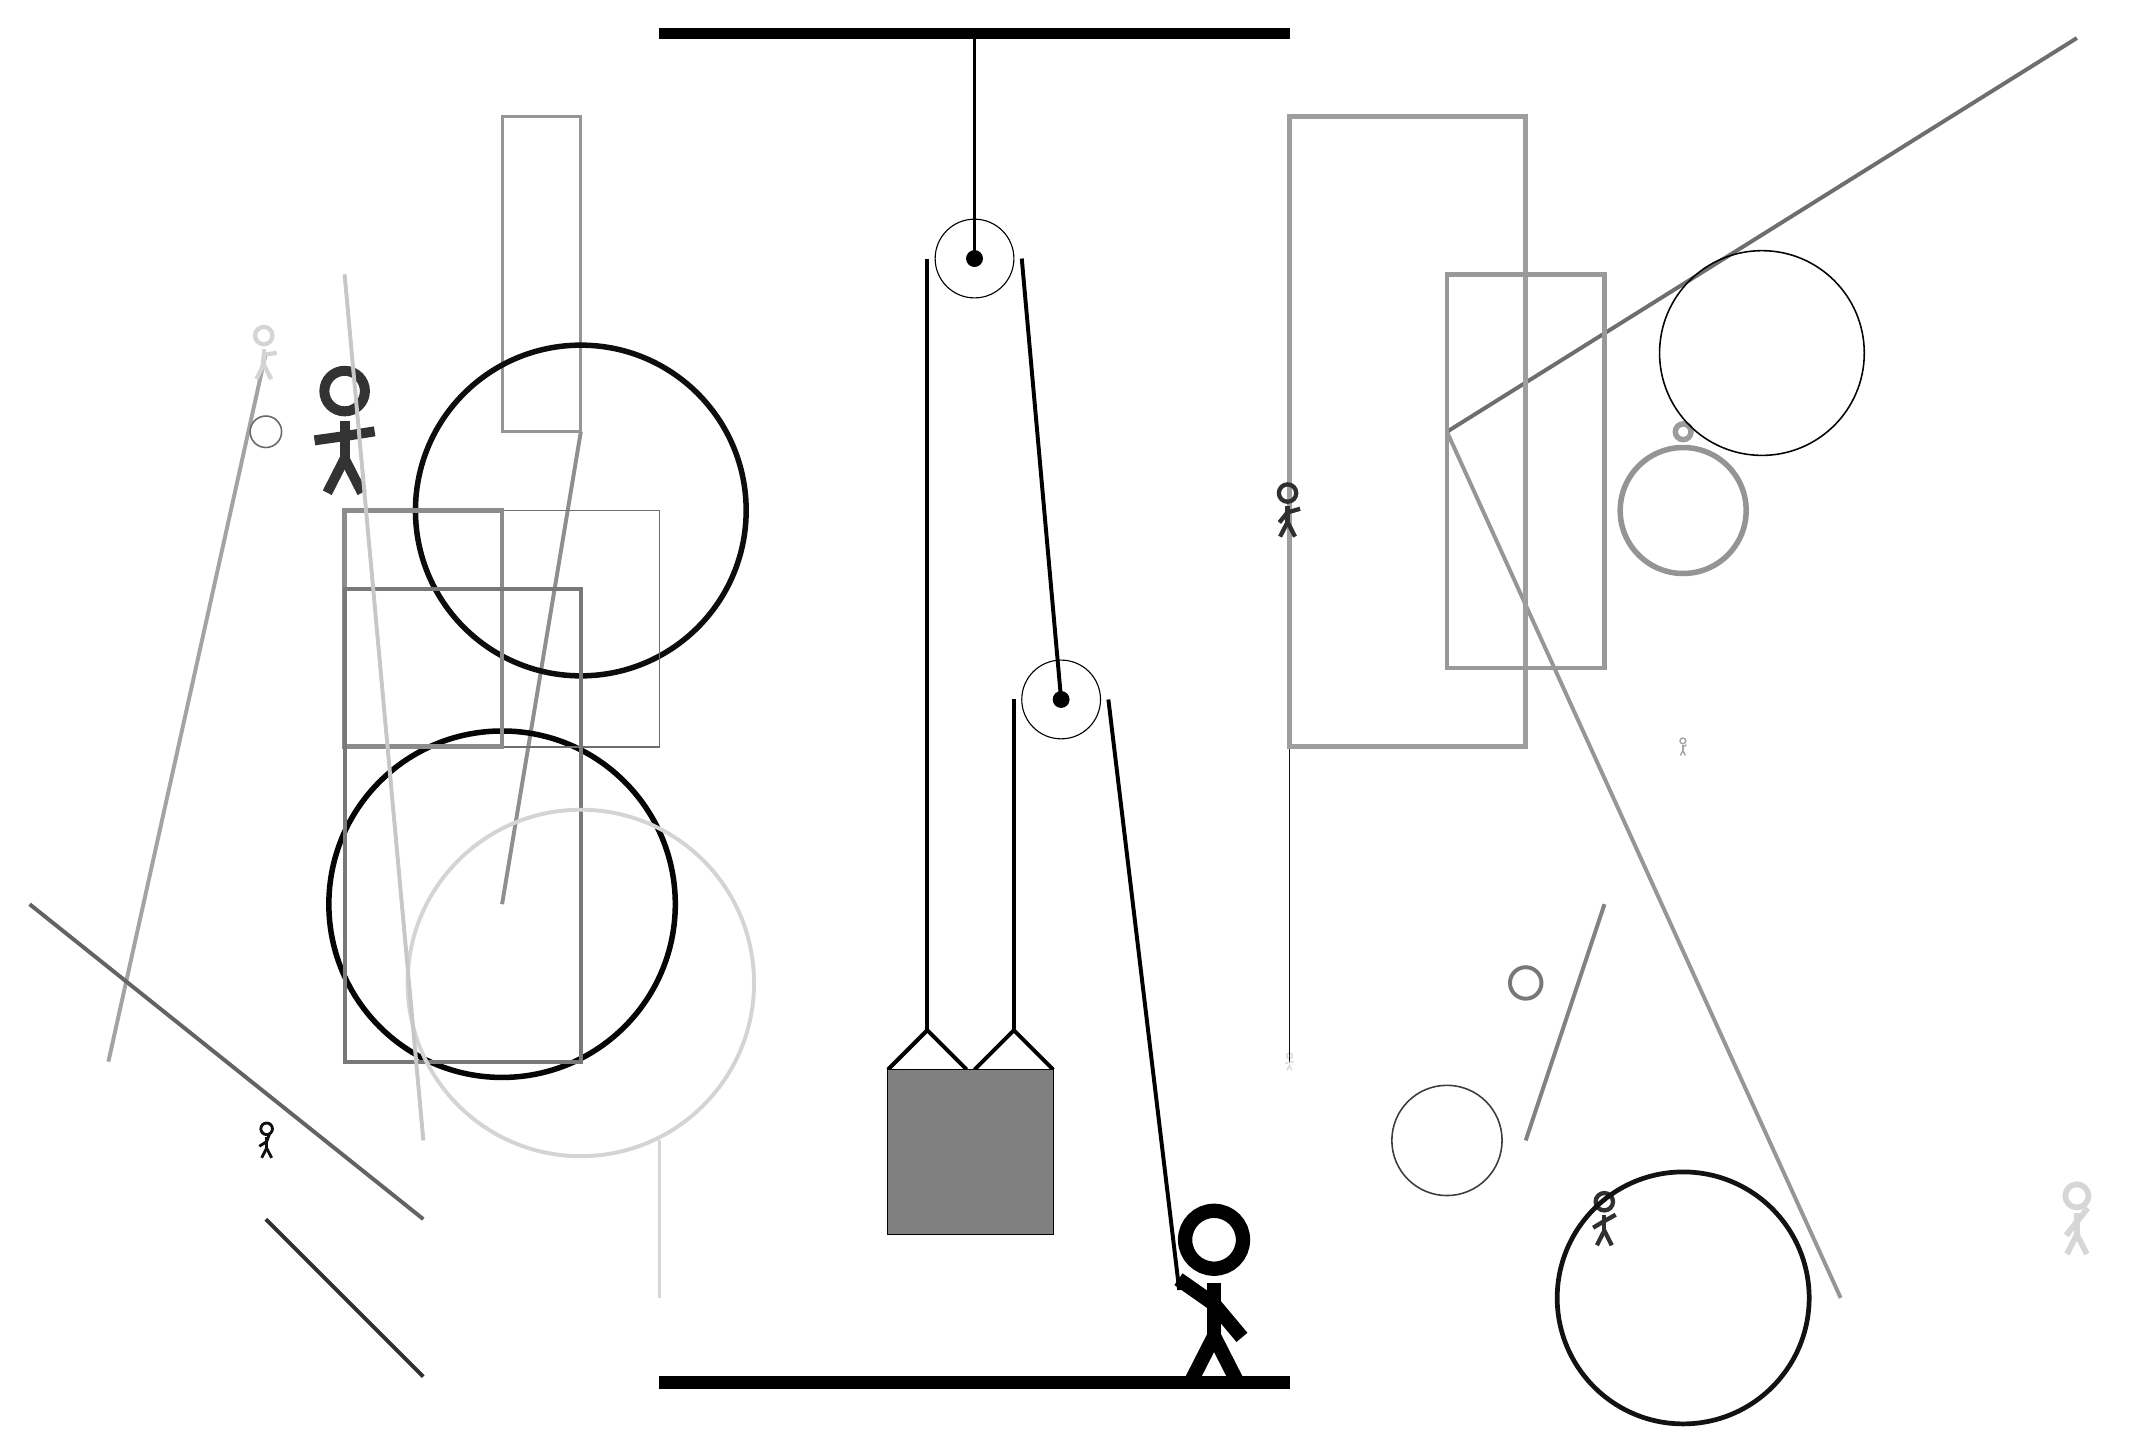
\begin{tikzpicture}
			%%%%% START %%%%%
			
			\draw[fill=black] (-2, 14) rectangle (6, 14.125);
			
			\draw[line width=0.5mm, color=black!41](8, 9) -- (13, -2);
			
			\node[line width=0.4mm, color=black!15] at (6, 1) {\Strichmaxerl[1][15][6]};
			\node[line width=0.4mm, color=black!80] at (-6, 9) {\Strichmaxerl[7][8][9]};
			\node[line width=0.3mm, color=black!94] at (-7, 0) {\Strichmaxerl[2][32][70]};
			\draw[line width=0.5mm, color=black!36](-7, 10) -- (-9, 1);
			\draw[line width=0.4mm, color=black!41] (-4, 13) rectangle (-3, 9);
			
			\draw[line width=0.2mm, color=black!94] (6, 10) rectangle (6, 1);
			
			\draw[line width=0.5mm, color=black!61](-5, -1) -- (-10, 3);
			\draw [line width=0.2mm, color=black!76](8, 0) circle (0.7);
			\draw[line width=0.5mm, color=black!44](-3, 9) -- (-4, 3);
			\draw[line width=0.5mm, color=black!57](8, 9) -- (16, 14);
			\node[line width=0.2mm, color=black!81] at (10, -1) {\Strichmaxerl[3][31][29]};
			\node[line width=0.4mm, color=black!35] at (11, 5) {\Strichmaxerl[1][89][36]};
			\draw [line width=0.7mm, color=black!98](-4, 3) circle (2.2);
			\draw [line width=0.5mm, color=black!53](9, 2) circle (0.2);
			\draw[line width=0.3mm, color=black!16] (-2, 0) rectangle (-2, -2);
			
			\draw [line width=0.7mm, color=black!42](11, 8) circle (0.8);
			\draw [line width=0.2mm, color=black!59](-7, 9) circle (0.2);
			\draw [line width=0.6mm, color=black!93](11, -2) circle (1.6);
			\draw [line width=0.7mm, color=black!39](11, 9) circle (0.1);
			\node[line width=0.7mm, color=black!17] at (-7, 10) {\Strichmaxerl[3][85][9]};
			\draw[line width=0.6mm, color=black!38] (6, 5) rectangle (9, 13);
			\node[line width=0.7mm, color=black!16] at (16, -1) {\Strichmaxerl[4][52][51]};
			\draw[line width=0.5mm, color=black!49](9, 0) -- (10, 3);
			\draw [line width=0.2mm, color=black!98](12, 10) circle (1.3);
			
			\draw[line width=0.6mm, color=black!40] (8, 11) rectangle (10, 6);
			
			\draw [line width=0.7mm, color=black!95](-3, 8) circle (2.1);
			\draw[line width=0.2mm, color=black!57] (-2, 5) rectangle (-4, 8);
			
			\draw[line width=0.6mm, color=black!45] (-4, 8) rectangle (-6, 5);
			
			\node[line width=0.4mm, color=black!81] at (6, 8) {\Strichmaxerl[3][51][16]};
			\draw[line width=0.5mm, color=black!53] (-3, 7) rectangle (-6, 1);
			
			\draw [line width=0.5mm, color=black!17](-3, 2) circle (2.2);
			\draw[line width=0.5mm, color=black!81](-7, -1) -- (-5, -3);
			\draw[line width=0.5mm, color=black!22](-6, 11) -- (-5, 0);
			
			\draw (2, 11.2) circle (0.5);
			\draw[fill=black] (2, 11.2) circle (0.1);
			\draw[thick] (2, 11.2) -- (2, 14);
			
			\draw (3.1, 5.6) circle (0.5);
			\draw[fill=black] (3.1, 5.6) circle (0.1);
			
			\draw[line width = 0.5mm]  (0.9, 0.9) -- (1.4, 1.4) -- (1.9, 0.9);
			\draw[line width = 0.5mm]  (2.0, 0.9) -- (2.5, 1.4) -- (3.0, 0.9);
			\draw[fill=black!50] (0.9, 0.9) rectangle (3.0, -1.2);
			
			\draw[line width = 0.5mm] (1.4, 11.2) -- (1.4, 1.4);
			\centerarc[line width = 0.5mm](2, 11.2)(0:180:0.6);
			\draw[line width = 0.5mm] (2.6, 11.2) -- (3.1, 5.6);
			\draw[line width = 0.5mm] (2.5, 5.6) -- (2.5, 1.4);
			\centerarc[line width = 0.5mm](3.1, 5.6)(0:180:0.6);
			\draw[line width = 0.5mm] (3.7, 5.6) -- (4.6, -1.9);
			
			\node at (5, -2) {\Strichmaxerl[10][-35][-50]};
			
			\draw[fill=black] (-2, -3) rectangle (6, -3.15);
			
			%%%%% END %%%%%
		\end{tikzpicture}
	\end{figure}	
\end{document}